% Formal regret definition (11/18 feedback item 4). Setting, safe set and executed path are defined in Sec. 3.
\subsection{Evaluation: simple regret}
\label{sec:regret}

\paragraph{Users.}
For evaluation a user is a unit vector $\theta^\ast$ ($\lVert\theta^\ast\rVert = 1$) with utility $u^\ast(s,k) = \theta^{\ast\top}\phi(s,k)$,
who answers a question $(i,j)$ with $P(i \succ j) = \sigma\bigl(\beta\,(u^\ast(s,i) - u^\ast(s,j))\bigr)$, $\beta = 5$.
After $n$ answers a method returns $\hat\theta_n$ (the Laplace posterior mean for Bradley--Terry methods, the DPO solution for DPO,
Sec.~\ref{sec:dpo}) and executes $\hat k_n(s)$ of Eq.~\eqref{eq:exec} among the safe candidates $\mathcal{C}(s)$ of Eq.~\eqref{eq:safe}.

\paragraph{Simple regret.}
The regret of that choice is the utility lost against the user's best safe candidate,
normalized by the utility range of the situation so that situations are comparable:
\begin{equation}
  r_n(s) = \frac{\max_{k \in \mathcal{C}(s)} u^\ast(s,k) \;-\; u^\ast\bigl(s,\hat k_n(s)\bigr)}
                {\max_{k \in \mathcal{C}(s)} u^\ast(s,k) \;-\; \min_{k \in \mathcal{C}(s)} u^\ast(s,k)}
  \;\in [0,1].
  \label{eq:regret}
\end{equation}
The reported number is its expectation over users and held-out test situations,
\begin{equation}
  \mathrm{SR}_n = \mathbb{E}_{\theta^\ast}\Bigl[\frac{1}{|\mathcal{S}_{\text{test}}|}
  \sum_{s \in \mathcal{S}_{\text{test}}} r_n(s)\Bigr],
  \label{eq:sr}
\end{equation}
where answers are only collected in query situations disjoint from the test situations
($\mathcal{S}_{\text{query}} \cap \mathcal{S}_{\text{test}} = \emptyset$; sizes in Sec.~\ref{sec:experiments}).
$\mathrm{SR}_n = 0$ for the oracle ($\hat\theta = \theta^\ast$);
a uniformly random safe candidate gives $\mathrm{SR} \approx 0.5$.

\paragraph{Why simple regret.}
Queries cost the user's attention but no driving utility, and what matters is the path the robot
executes afterwards. The objective is therefore best-arm identification (simple regret) rather
than cumulative regret over the queries. EUBO~\citep{astudillo2023qeubo} is one-step Bayes-optimal
for exactly this objective under noise-free answers, which motivates its use.
Fig.~\ref{fig:regret} plots $\mathrm{SR}_n$ against the number of queries $n \in \{0,2,5,10,20\}$.

\paragraph{Variants used elsewhere.}
\emph{Closed loop:} at every 0.8\,s re-planning step $t$ of a drive, Eq.~\eqref{eq:regret} is evaluated
on that step's safe set $\mathcal{C}(s_t)$ and averaged over the steps of the episode (step regret).
\emph{Candidate generators:} to compare two generators $A$ and $B$ on the same situation, the max and min
in Eq.~\eqref{eq:regret} are taken over $\mathcal{C}_A(s) \cup \mathcal{C}_B(s)$ (union regret), so a generator
whose candidates miss what the user wants is penalized even when it picks its own best;
the per-generator regret of Eq.~\eqref{eq:regret} is not comparable across generators.
\emph{Pilot:} with real participants $\theta^\ast$ is unknown; the measurable proxy is the share of
held-out (test-block) answers that $\hat\theta$ predicts.

% Figure (utils/plot_regret_curves.py -> reports/fig_regret.pdf)
\begin{figure}[t]
  \centering
  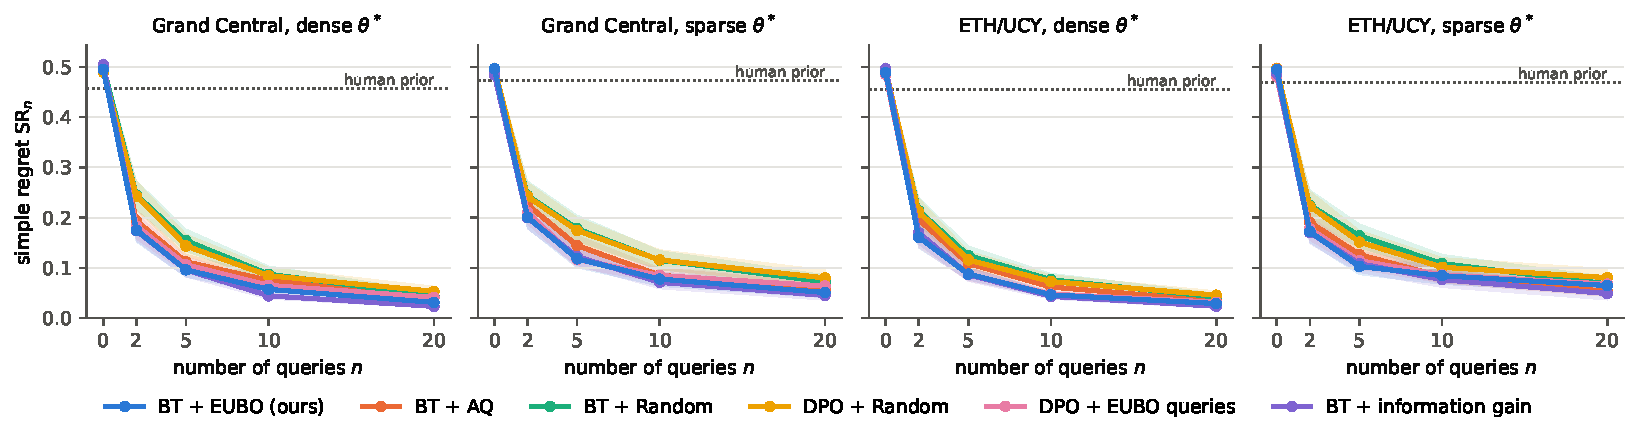
\includegraphics[width=\linewidth]{figures/fig_regret.pdf}
  \caption{Simple regret $\mathrm{SR}_n$ (Eq.~\ref{eq:sr}) on held-out situations against the number of
  A/B queries. Shaded: 95\% bootstrap CI over 200 synthetic users. Dotted: human prior only; the oracle is 0. BT: Bradley--Terry (Laplace); DPO: Sec.~\ref{sec:dpo}.}
  \label{fig:regret}
\end{figure}
